\section{Evaluation}
\label{sec:eval}

We evaluate RCuckoo by directly comparing its performance in terms of
latency and throughput with other state-of-the-art disaggregated key
value stores. We substantiate our design decisions through a series of
micro-benchmarks. Specifically, we measure throughput as a function of
hashing locality, covering read threshold, and choice of search
algorithm.

\section{Implementation}

Our implementation of RCukcoo consists of a of 8.7k C++
implementation and a 12k line Python implementation which
simulates RDMA. Both implementations will be made available
on Github.  All results reported in Section~\ref{sec:eval}
are from the C++ implementation. At the time of writing only
the python implementation includes support for delete
operations, and extent entries. As such all C++ results are
for inserts, reads, updates and inlined table operations.
RCuckoo is designed for ConnectX-5 NICs. It uses OFED-4.9
which supports experimental verbs for atomic masked CAS and
device mapped memory. 


\begin{figure*}[ht]
    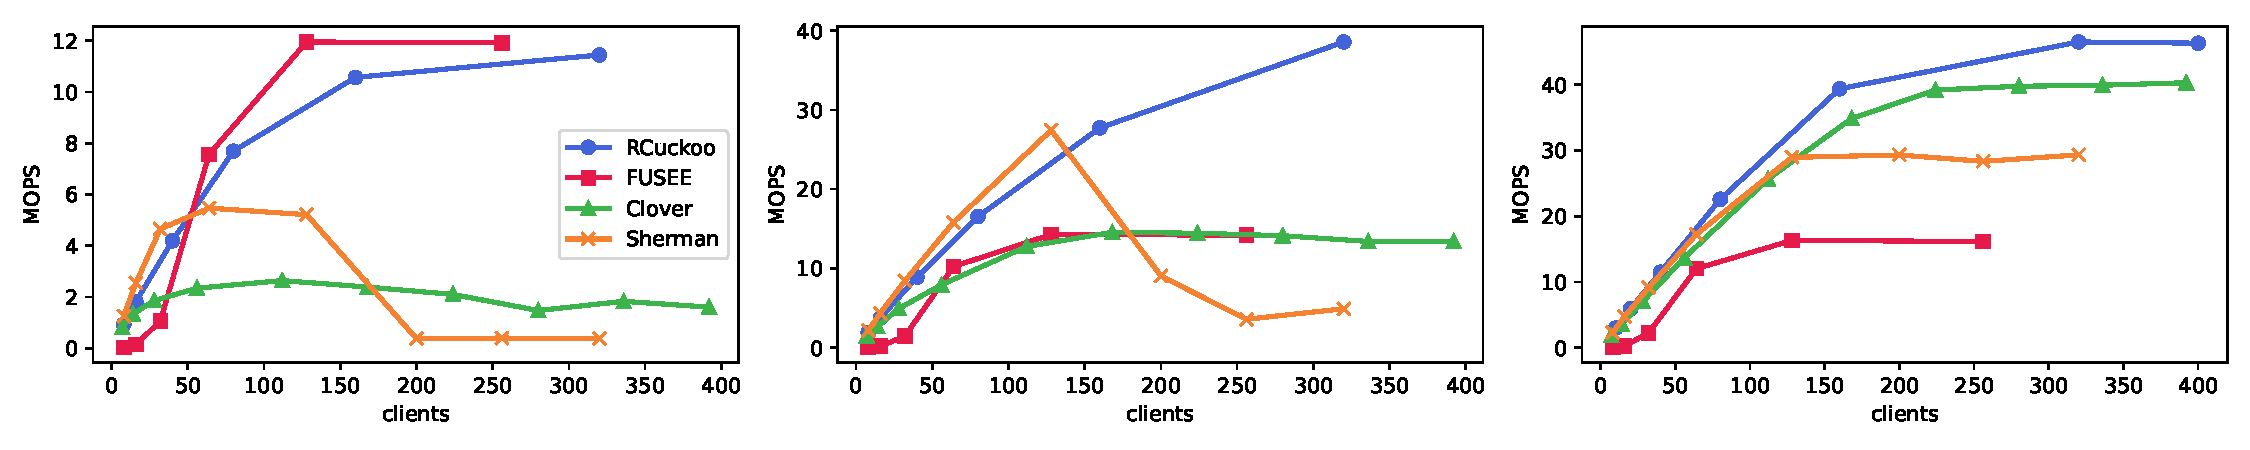
\includegraphics[width=0.99\linewidth]{fig/hero_ycsb_throughput.pdf}

    \caption{Rcuckoo throughput vs workload (Zipf $\theta$=0.99). A) YCSB-A 50\%
    read 50\% update. B) YCSB-B 95\% read 5\% update. C)
    YCSB-C 100\% read}
    \label{fig:ycsb_throughput}
 \end{figure*}

\begin{figure*}[ht]
    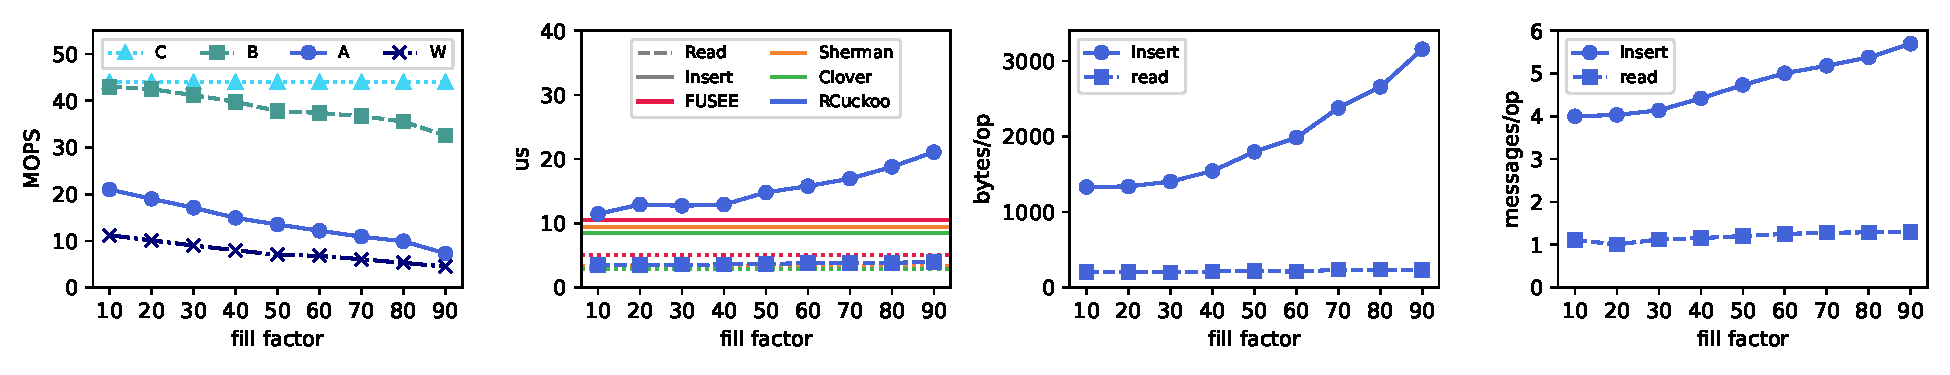
\includegraphics[width=0.99\linewidth]{fig/hero_ycsb_fill.pdf}

    \caption{Rcuckoo's insert and read performance as a
    function of fill factor. A) Workload throughput. B)
    Median operation latency. C) Average operation size. D)
    Average messages per operation. Figures B through D are
    YCSB-A.}

    \label{fig:ycsb_fill}
\end{figure*}

% \begin{figure}[ht]
%     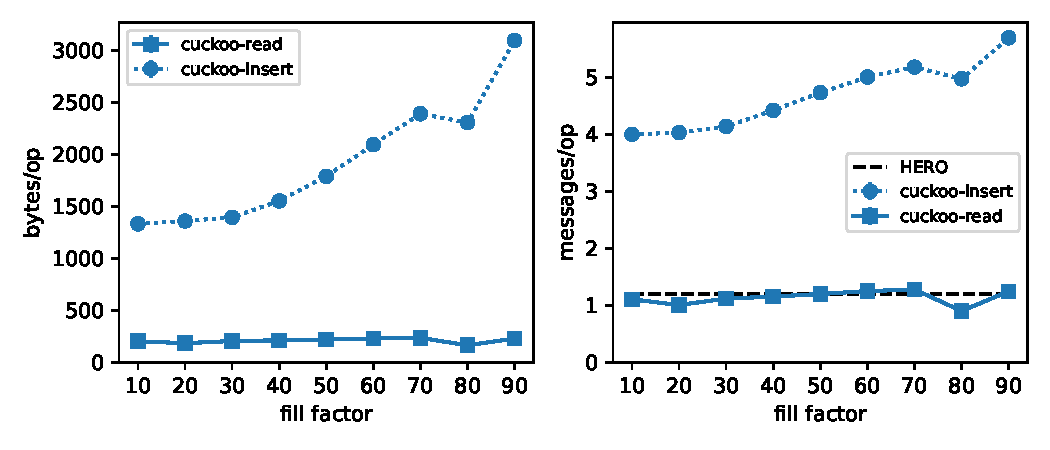
\includegraphics[width=0.99\linewidth]{fig/hero_ycsb_fill_ops_bw.pdf}
%     \caption{YCSB-A workload messages and bandwidth per operation as a function of fill factor}
%     \label{fig:ycsb_fill_ops_bw}
% \end{figure}

\begin{figure}[ht]
    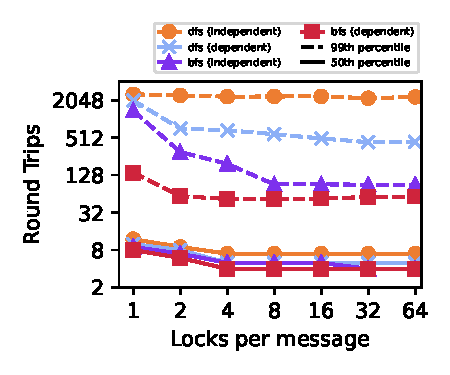
\includegraphics[width=0.99\linewidth]{fig/search_dependence.pdf}

    \caption{ Search function performance with independent
    and dependent hashing.}

    \label{fig:search_dependence}
\end{figure}

\subsection{Testbed}

We conduct our evaluation on an 11-node cluster of dual-socket Intel
machines. Each CPU is an Intel Xeon(R) E5-2650 clocked at
2.20~GHz. Each machine has 256~GB of RAM with 128~GB per NUMA
node. All machines have a single dual-socket ConnectX-5 attached to a
100-Gbps Mellanox Onyx switch. In our RCuckoo experiments we use one
sever as the passive memory server and the rest a client machines
spreading out client threads evenly across machines.

\subsection{Comparision systems}

We compare RCuckoo against three recent key-value stores with
different designs.  While none have the same feature set as RCuckoo,
each represents an apt comparision point for different aspects.

\subsubsection{FUSEE}

FUSEE is a key-value store designed for full
disaggregation~\cite{fusee}.  It is built on top of RACE~\cite{race}
with extensions to support replication in the face of contention.
While RACE represents a more direct comparison to RCuckoo, no open
source implementation of RACE is available.  Instead, we deploy FUSEE
with a single memory node to effectively remove the overhead of
replication.  FUSEE/RACE hashing uses fixed-sized 64-bit index entries
to in order to employ RDMA compare-and-swap operations for updates. As
such, RACE-based systems cannot store key-value pairs in the index
table itself and require a second round trip even for reads of small values.
%on reads to recover
%extent entries which contain full key value pairs.

\subsubsection{Clover}

Clover is a key-value store designed for remote persistent memory. It
does not support full disaggregation; instead, its index structure is
managed by CPU cores on a metadata server. However, its
persistent-memory updates are implemented using by one-sided
operations. Clover uses index caching to optimize reads. Clover reads
are self verifying unlike FUSEE as clover entries contain a NULL
terminating pointer if the entry is valid. When re-reading key-value
entires clover can achieve close to RDMA line rate as it directly
reads the entry without negotiating with the index. In contrast to
prior work which has compared with Clover~\cite{fusee} we do not force
clients to read from the index on each read and allow it to take
advantage of it's caching algorithm.

\subsubsection{Sherman}

Sherman is a B-tree designed for remote memory and high
write throughput. Sherman clusters are not fully
disaggregated.  Each node in a sherman cluster has many CPU
cores, and a single memory core. Unlike the other systems
Sherman is cluster based, and does not support a having
isolated memory machines. All machines are equal nodes in a
cluster and run both a memory controller and client threads.
As such Sherman does not see bandwidth bottlenecks the other
systems experience as the requests are partitioned across
machines.  Sherman's memory core is responsible for
servicing allocation RPC calls from clients. Sherman is
similar to RCuckoo in that it uses locks to guard access.
However, it assumes that colocated clients can resolve lock
contention locally and clients colocated with their segment
of the B-Tree can perform local operations. These
assumptions enable sherman to have high performance under
contention even though it uses locks and manages a more
complex data structure than the unordered key-value stores.
While Sherman does not meet the fully disaggregated model it
does provide a good comparison for RCuckoo as it is the only
other system to use locks in remote memory.


% \subsubsection{Clover}
% \todo{insert a short clover description}

\subsection{System Performance}

\textbf{YCSB Throughput:} Figure~\ref{fig:ycsb_throughput} shows
the throughput of FUSEE, Sherman, Clover and RCuckoo for
YCSB workloads on a zipf (0.99) distribution. YCSB-A is a
50\% read 50\% update workload.  YCSB-B is 95\% read and 5\%
update, and YCSB-C is 100\% read.  In each experiment
clients fill the hash table from empty to 90\% full on
tables with 100M 32bit keys and 32bit values.

On YCSB-A RCuckoo outperforms FUSEE largely due to it's
requirement for one fewer round trips per operation. RCuckoo
hit's a bottleneck on this skewed update workload at
approximately 160 clients due to lock contention on hot
keys. Sherman performs in-line with RCuckoo until ~5MOPS.
Updates to Shermans B-Tree have larger critical sections
than RCuckoo leading to the performance bottleneck. On
uniform distributions Sherman and RCuckoo perform similarly
on YCSB-A. Clover suffers the most on YCSB-A. Each update to
a key causes other clients to re-read the key prior to
updating.

On read mostly and read only workloads (YCSB-B,C
respectively) RCuckoo has a distinct advantage over FUSEE as
it completes each read in a single round trip, rather than
two, it sees a further benefit from summarizing most reads
into a single packet (Section~\ref{sec:read_threshold}).
Sherman has an advantage on read mostly workloads as it can
directly read from the B-Tree in a single round trip rather
than resolving a pointer. On YCSB-B it hits the same
bottleneck as before due to hot keys. On YCSB-C it performs
similarly to RCuckoo, however Sherman has a more complex
read algorithm than RCuckoo leading to an earlier
bottleneck. Clover performs similar to FUSEE on read mostly,
and is the most competitive with RCuckoo on read only.
Clovers reads are very similar to RCuckoo's when it can use
it's cached index. We believe that with more aggressive
tuning Clovers read only performance would be nearly
identical to RCuckoo as the semantics are very similar.


\textbf{Insert Performance:}
%%
By default YCSB-A,B,C use updates. RCuckoo's insert
algorithm is it's most complex and bandwidth intensive
component. In this section we evaluate RCuckoo's insert
performance using modified YCSB. We run inserts rather than
updates, so YCSB-A is 50\% read, 50\% insert. We add an
additional benchmark \textit{YCSB-W} which is insert only.
Figure~\ref{fig:ycsb_fill}(a) shows the throughput
of each workload in response to the tables fill size with
400 clients. As the cuckoo table fills, cuckoo paths are
longer leading to more contention, and more bandwidth usage
to perform covering reads. In each case (except YCSB-C)
RCuckoo's performance drops with relation to fill factor. In
the case of insert only (YCSB-W) RCuckoo's performance drops
from 11.5 to 4.5 MOPS. We measured FUSEE's insert only
performance at 9.1 MOPS which is invariant to fill factor.
While RCuckoo is slower on insert only we note that insert
only is an uncommon workload~\cite{facebook-memcached}.

We additionally measure latency, operation size, and
messages (rdma packets) per operation
(Figure~\ref{fig:ycsb_fill}(b-d)). In all cases inserts are
more expensive as the table fills, but have little impact on
read performance. As the table fills, cuckoo paths grow in
length causing an increase both in bandwidth consumption per
operation but also latency as additional round trips are
required to find valid cuckoo paths. We report latency
values for insert and read for each project. These values
were not collected under load and represent near min values.
For all projects except FUSEE read latency is nearly the
same (single rdma round trip). Insert times vary. Clover and
Sherman use two sided RDMA RPC's for insert, both perform
allocations and set up metadata for the requesting client.
FUSEE has the lowest fully disaggregated latency.

\subsection{Fault Tolerance}
\begin{figure}[ht]
    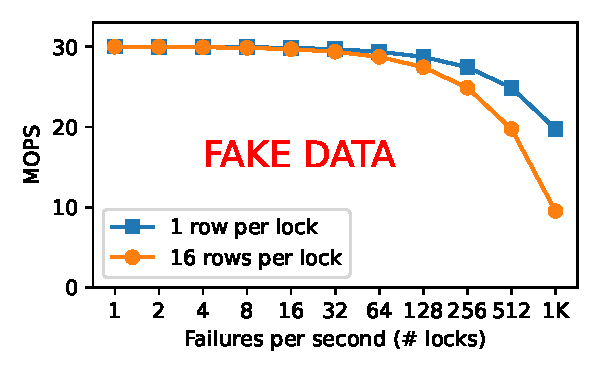
\includegraphics[width=0.99\linewidth]{fig/failure_throughput.pdf}
    \caption{Throughput vs Failure Rate}
    \label{fig:failure_throughput}
\end{figure}

Failures in critical sections leave locks set and reduce
overall system performance to lower until the lock is
reclaimed and the table is repaired. We measure RCuckoo's
performance in the face of failures by injecting. A
\textit{Failure Client} emulates the failure of a client in a
critical section by performing an insertion but only issuing
a randomly truncated set of packets when updating and
unlocking the table. This randomly leaves the table in one
of the three recovery states and leaves some locks set. In
our experiment the table is filled to 80\%, clients are set
to a ycsb-a workload, and the failure client is given a
maximum rate at which it will inject faults.

Figure~\ref{fig:failure_throughput} Shows the degradation in
throughput as the failures per second increases. The more
rows a lock protects the larger the failures impact and time
to triage and repair the failure. The performance impact of
a few number of failures per second is low which is ideal
considering that failures in RDMA clusters are relatively
rare. Rcuckoo can still operate with thousands of failures
per second while RDMA can only establish approximately 1.4K
connections per second using state of the art
techniques~\cite{xrdma}.

\subsection{Dependent hashing and search}

Hash dependence and search function choice have the highest
impact on RCuckoo's performance. Dependent hashing reduces
the probability locks are scattered throughout the table
which enables RCuckoo to combine lock requests into a few
masked CAS messages. Simultaneously search function choice
dramatically affects the length of cuckoo paths. BFS
produces much shorter paths than
DFS~\cite{cuckoo-improvements,pilaf,cuckoo}.
Figure~\ref{fig:search_dependence} illustrates the effect of
search function and dependent hashing on RCuckoo's inserts.
We vary the number of locks per message to demonstrate the
effect of path length and show why masked cas plays an
important role in RCuckoo's performance. We measured both
the median, and 99th percentile round trips per request on a
table with 100M entries. We fille the table to 85\% and then
executed insert operations to 95\%.

DFS with no hash dependence has extremely poor performance
at it's tail, taking over 2K round trips to complete. Both
at it's median and 99th percentile it sees only small
benefits from setting multiple locks per request as the
locks are scattered throughout the table. DFS with
dependence has far lower tail latency, and improves the
number of locks which can be acquired per message, however
it still constructs long rather than minimum length paths.
BFS with dependence provides the best performance and gains
the most from setting more locks per request. At 64 locks
per request it has 7.5x lower round trips at it's 99th
percentile and 4 rather than 5 round trips on average. We
found that A* search provided the same minimal path length
as DFS with slightly better locality. It's performance
against BFS was only superior at fill factors above 95\% and
lower elsewhere due to a higher runtime cost on short paths.



% Hash function locality hash a major impact in rcuckoo's
% performance.  Acquiring locks can only be done in a few
% round trips when the locks are clustered together tightly in
% the lock table.  Furthermore, the search function used to
% determine the cuckoo path has a large impact on the locality
% of the locks necessary to lock the path. We evaluate
% dependent hashing and independent hashing as well as random
% and a* search. We measure the number of round trips required
% for each control as a function of the number of locks which
% can be acquired per round trip.

% Figure~\ref{fig:search_dependence} shows the performance
% improvements gained by both locality hashing and A* search.
% In this experiment the table is filled from 0 to 90\% full
% with a ycsb-w workload. We measure the 99th percentile of
% round trips for these workloads. Random search with
% independent hashing leads to a large number of round trips
% as locks are scattered throughout the table. RDMA masked CAS
% operation do little here to reduce the round trips as they
% can rarely aquire more than one lock in a round trip. With
% dependent hashing and random search RDMA CAS operation are
% almost sufficient to reduce round trips, however the absolute
% number of locks required per insert is high which leads to
% greater contention. A* search with dependent hashing has
% cuckoo paths that are both short, and clustered together.


\begin{figure*}[t]
    \centering
    \begin{subfigure}{0.3\linewidth}
        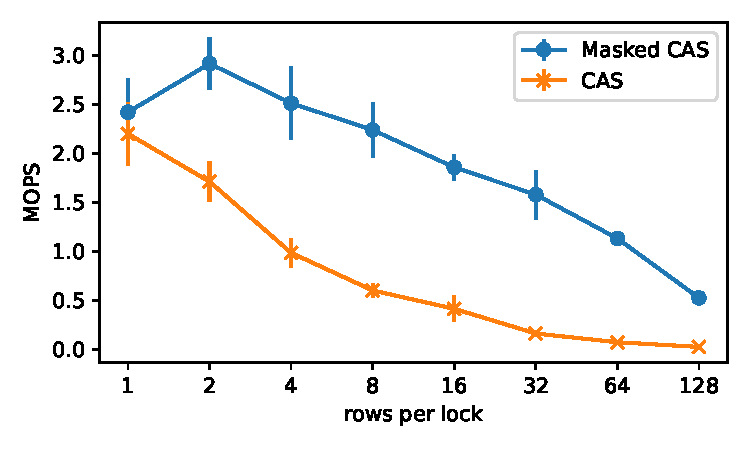
\includegraphics[width=0.99\linewidth]{fig/masked_cas_lock_size.pdf}
    \end{subfigure}
    \begin{subfigure}{0.3\linewidth}
        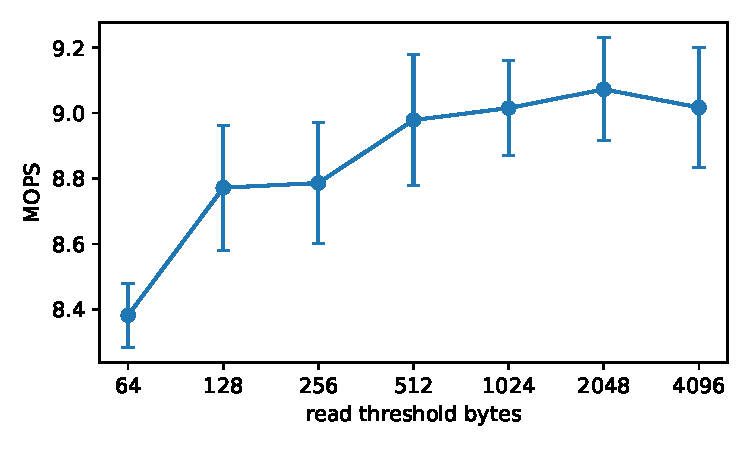
\includegraphics[width=0.99\linewidth]{fig/read_size.pdf}
        % \label{fig:hash_factor}
        % \caption{}
    \end{subfigure}
    \begin{subfigure}{0.3\linewidth}
        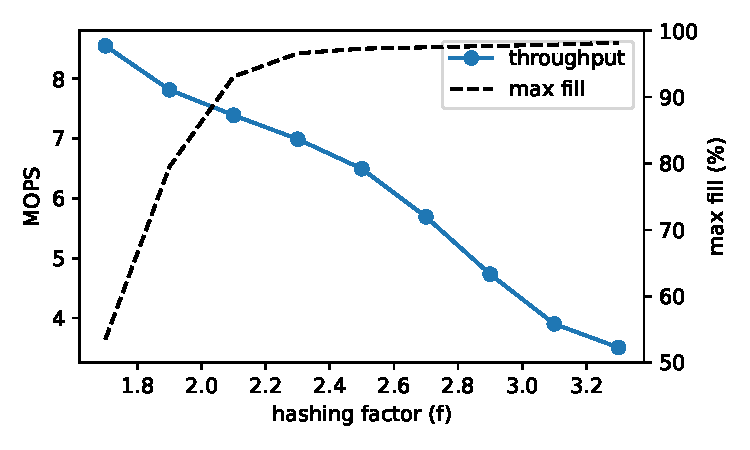
\includegraphics[width=0.99\linewidth]{fig/factor.pdf}
        % \label{fig:hash_fill}
        % \caption{}
    \end{subfigure}.
    \vspace{-1em}
    \caption{
    \textbf{(a)} Masked CAS vs Unmasked CAS throughput.
    \textbf{(b)} Read threshold vs throughput.
    \textbf{(c)} Exponential factor relation to max fill in cuckoo hash.
    }
    \label{fig:performance_breakdown}

\end{figure*}

\subsubsection{Masked CAS}

Under contention masked CAS operations provide a significant
performance improvement. We measure it's benefit in terms of
throughput by comparing it with default CAS. In the
default case, when acquiring locks clients set the lock bits
for the locks they require and set all other bits in the cas
to 0. If the cas fails the current state of the lock table
over that range is returned as a result to the client and
the client tries to aquire their locks again using the
updated state of the lock table. Masked compare and swaps
are issued with the minimal mask required to set the locks.

Figure~\ref{fig:performance_breakdown} shows the improvement
gained by masked CAS. Default CAS operations perform better
with fewer rows per lock, as the probability of a lock being
set within the 64bit range is at its lowest. At higher rows
per lock CAS suffers from failed lock acquisitions from both
contested locks and due to a lack of synchronization. In
contrast masked CAS sees an improvement when two rows per
lock are used, as more second search attempts succeed, and
only suffers from direct lock contention as the rows per
lock increase.


\subsection{Hash Function Factor $f$}

Low hash factors $f$ have higher performance due to better
locality at the tradeoff of their maximum fill factor. The
relationship between $f$ and performance is nearly linear,
while the relationship between $f$ and fill factor is
exponential. Figure~\ref{fig:performance_breakdown}(c) shows
the relationship between $f$, the max fill rate, and insert
performance. These numbers were collected on an insert only
workload with 100 million table entries. We choose an $f$ of
2.3 in practice as it has the highest product of fill factor
and throughput.

\subsection{Read Threshold Performance}
\label{sec:read_threshold}
As described in section ~\ref{sec:reading} rcuckoo uses a
read threshold to capture both hash locations if the
locations are within a defined read threshold.
Figure~\ref{fig:performance_breakdown}(b) shows the
performance gains from increasing the read threshold. Here
each row is 64 bytes so our minimum threshold of 64 ensures
two packets are issued for each read request. We limit the
number of clients to 40 so that their is plenty of bandwidth
to support the inflated reads. Higher read thresholds trade
off network bandwidth for operation latency. When bandwidth
is plentiful large windows can improve throughput but up to
8\%.

% \begin{figure}[ht]
%     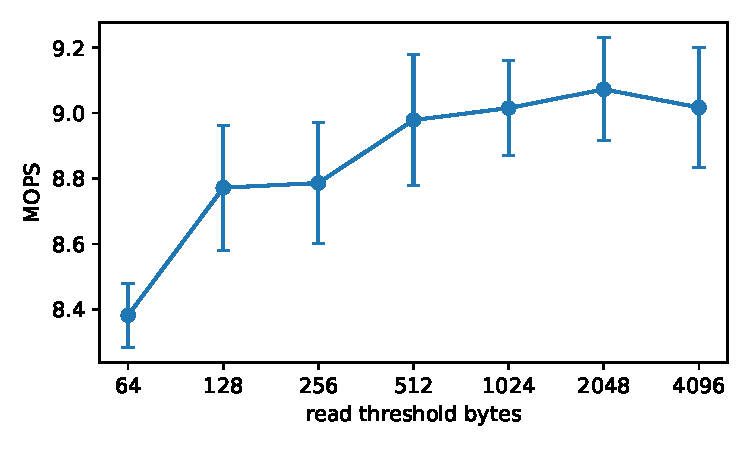
\includegraphics[width=0.99\linewidth]{fig/read_size.pdf}
%     \caption{Read Threshold vs Throughput}
%     \label{fig:read_threshold}
% \end{figure}


\subsection{Entry Size}
\begin{figure}[ht]
    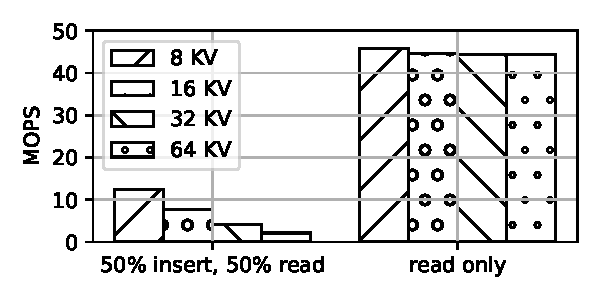
\includegraphics[width=0.99\linewidth]{fig/entry_size.pdf}
    \caption{Throughput vs KV entry size}
    \label{fig:entry_size}
\end{figure}

Key value pairs embedded directly in the index enable single
round trip reads, at the cost of inflating the bandwidth of
operations. We run a 50\% read 50\% insert and a read only
workload to illustrate the overhead of larger entries.
Figure~\ref{fig:entry_size} shows the effect of key value
pair size on operation throughput. Insert quickly saturates
the network bandwidth. At 16 byte KV entries the network
bandwidth is fully absorbed at 8MOPS. Reads which have lower
bandwidth requirements see very little chance in throughput
across entry sizes. We suggest that known read heavy
workloads should use inlined entries as reads see a large
boost in performance. Update operations are similarly
unaffected by entry size up to 64 bytes. 

% Our design choice
% in embedding KV pairs is motivated by networking trends
% which suggest that 800 GBPS and higher network speeds will
% be available in the coming years. While round trip latency
% is expected to remain largely the same.

\subsection{Search Success}
\label{sec:search_success}
\begin{figure}[ht]
    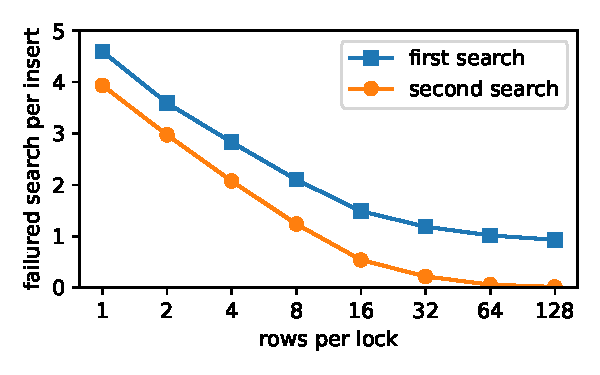
\includegraphics[width=0.99\linewidth]{fig/search_success_lock_size.pdf}
    \caption{Failure rate of search algorithms vs lock size under high contention}
    \label{fig:search_success}
\end{figure}

RCuckoo's two stage search algorithm is designed to improve
the probability that an insert will be successful given that
a clients local cache is out of sync. To demonstrate the
effectiveness of our two stage search strategy we measure
the success rate of our searches under high contention. With
400 concurrent clients we fill a small table (10M entries)
up to 85\% prior to measuring success rate in order to
maximize cuckoo path length. Figure~\ref{fig:search_success}
shows the failure rate of both search stages. The first
search is the success rate of a search based entirely on
cached information. The second search is the success rate of
our restricted search performed after acquiring locks. We
measure the response of both as a function of lock size.
Given 1 row per lock the failure rate of both searches is
over 4 as the local cache is almost always out of sync, and
retries are not guaranteed to be synchronized. As lock
granularity grows the frequency of second search success
drops dramatically. At 64 rows per lock our second search
succeeds 95\% of the time even when the cached search fails
at a rate of 99\% per insert.



